\chapter{Тестирование и апробация}\label{ch4}

Данная глава посвящена тестированию разработанных компонентов
и апробации системы на боевых контурах платформы.

\section{Тестирование компонентов системы}\label{sec:testing}

\subsection{Интеграционные тесты auth-jwt}\label{subsec:ch4-integration-tests}

Для интеграционного тестирования auth-jwt разработан
предметно-ориентированный язык (Domain-Specific Language, DSL),
позволяющий описывать тесты лаконично
даже для сложного функционала.
DSL состоит из трёх слоёв:
прямые операции с базой данных,
операции через HTTP API
и операции с секретами в Vault.

В листинге~\ref{lst:integration-test} приведён
пример теста генерации токена.

\begin{lstlisting}[language={[Sharp]C},
  label={lst:integration-test},
  caption={Интеграционный тест генерации токена с использованием DSL}]
[TestMethod]
public async Task GenerateToken_ValidParameters_TokenGenerated()
{
    // Arrange: создание клиента через DSL
    var client = BuildAuthClient(TestClientId,
        tokenPolicies: [BuildPolicy(TestPolicy,
            permissions: ["ReadSomething"],
            allowTenantHeader: true)]);
    await AuthClientsDb.CreateAsync(client);
    var k8sToken = GetK8STokenFake(TestClientId);

    // Act: запрос токена через HTTP
    using var content = JsonContent.Create(
        new ClientTokenRequest {
            ClientId = TestClientId,
            Tenant = "testTenant",
            Policy = TestPolicy });
    var response = await ServicesProject.SendAsync<TokenResponse>(
        "/token", HttpMethod.Post, content, token: k8sToken);

    // Assert: проверка claims и метрик
    var jwt = ReadJsonWebToken(response.Token);
    Assert.AreEqual(TestClientId, jwt.Subject);
    AssertClaim(jwt, MindboxJwtConstants.TenantClaim, "testTenant");

    var metricValue = _tokenIssuedCounter
        .WithLabels(TestClientId, TestPolicy, "testTenant").Value;
    Assert.AreEqual(1, metricValue);
}
\end{lstlisting}

Тест читается как спецификация:
создать клиента с политикой,
запросить токен,
проверить содержимое и метрику.
Вспомогательные методы \texttt{BuildAuthClient},
\texttt{BuildPolicy}, \texttt{GetK8STokenFake}
скрывают подготовку инфраструктуры,
а \texttt{AssertClaim}~--- типовые проверки JWT.
Помимо содержимого токена, тест проверяет,
что метрика Prometheus была инкрементирована~---
это гарантирует наблюдаемость.

\begin{figure}[h]
  \centering
  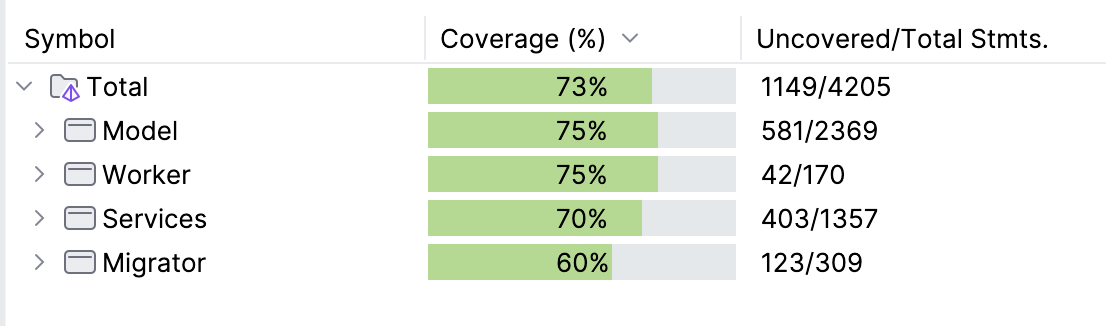
\includegraphics[width=\textwidth]{diagrams/img/test-coverage.png}
  \caption{Покрытие кода интеграционными тестами auth-jwt}
  \label{fig:test-coverage}
\end{figure}

\subsection{E2E-тесты оператора}\label{subsec:ch4-e2e-tests}

Для end-to-end тестирования оператора используется
фреймворк Ginkgo~--- BDD-фреймворк для Go.
Тесты запускают Kind-кластер (Kubernetes в контейнере),
разворачивают оператор с fake backend
и проверяют реальное поведение системы.

В листинге~\ref{lst:e2e-test} приведён сокращённый тест,
проверяющий, что удалённые из CR токены
остаются в Secret до истечения срока действия.

\begin{lstlisting}[language=Go,
  label={lst:e2e-test},
  caption={E2E-тест: удалённые токены остаются в Secret до истечения TTL}]
It("deleting tokens from CR does not remove from secret "+
    "until expiration", func() {

    By("applying valid AuthJwtConfig")
    cmd.ApplyAuthJwtConfig(authjwtv1.AuthJwtConfig{
        Spec: authjwtv1.AuthJwtConfigSpec{
            Contour:    "stable",
            SecretName: secretName,
            Tokens: []authjwtv1.TokenSpec{{
                Name:   "api-token",
                Policy: authjwt.FakeShortLivedPolicy,
            }},
        },
    })

    By("awaiting first reconcile")
    waitForFirstReconcile(clientNS, clientName)

    By("removing tokens from spec")
    cmd.ApplyAuthJwtConfig(authjwtv1.AuthJwtConfig{
        Spec: authjwtv1.AuthJwtConfigSpec{
            Contour: "stable", SecretName: secretName,
            Tokens:  []authjwtv1.TokenSpec{},
        },
    })

    By("checking token remains in secret")
    Consistently(func(g Gomega) {
        secret, _ := cmd.GetAuthSecretData(clientNS, secretName)
        g.Expect(secret.Tokens).To(HaveKey("api-token"))
    }, 2*time.Second, 200*time.Millisecond).Should(Succeed())

    By("waiting for secret removal after expiration")
    Eventually(func(g Gomega) {
        secret, _ := cmd.GetAuthSecretData(clientNS, secretName)
        g.Expect(secret.Tokens).NotTo(HaveKey("api-token"))
    }).Should(Succeed())
})
\end{lstlisting}

Тест использует две ключевые конструкции Ginkgo:
\texttt{Consistently}~--- утверждает, что условие выполняется
непрерывно в течение заданного интервала;
\texttt{Eventually}~--- ожидает выполнения условия с таймаутом.

\begin{figure}[h]
  \centering
  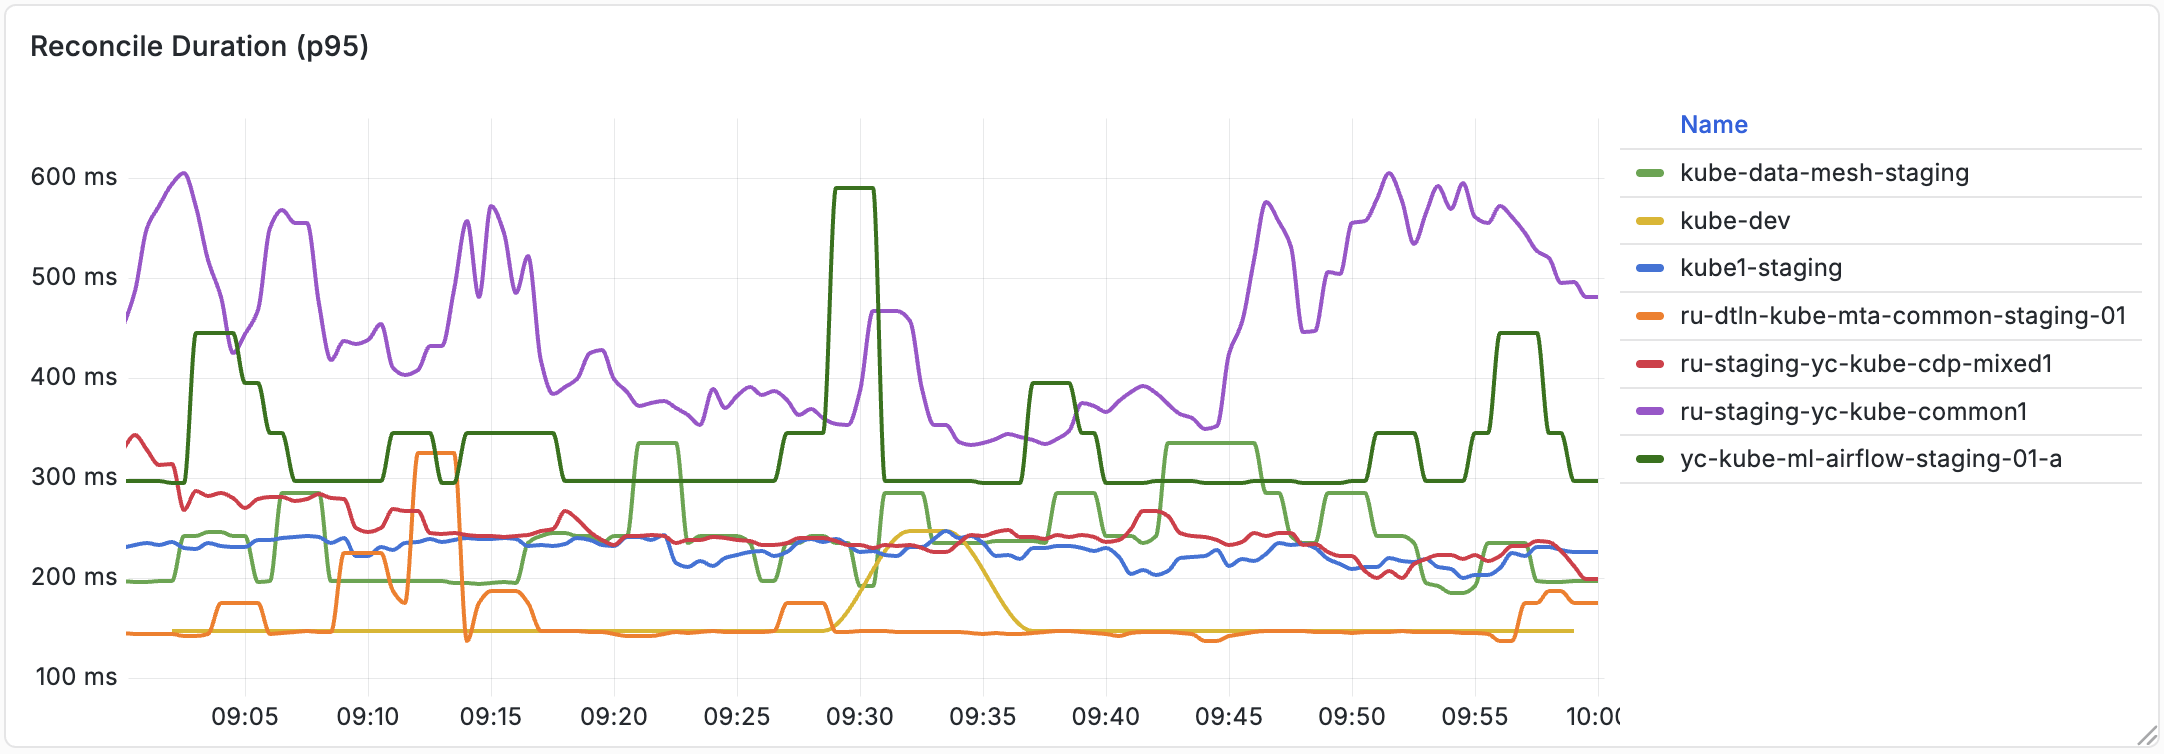
\includegraphics[width=\textwidth]{diagrams/img/operator-reconcile.png}
  \caption{Время реконсиляции оператора на контуре Alpha}
  \label{fig:reconcile-grafana}
\end{figure}

\subsection{Тестирование клиентской библиотеки}\label{subsec:ch4-lib-tests}

Библиотека Mindbox.Authentication покрыта двумя уровнями тестов.
Юнит-тесты проверяют каждый компонент в изоляции:
кеширование и инвалидацию токенов,
вычисление буфера для различных TTL,
построение ключа кеша,
генерацию политик авторизации
и корректность конфигурирования.
Интеграционные тесты запускают полноценный экземпляр ASP.NET Core
через \texttt{TestWebApplicationFactory}
и проверяют end-to-end сценарии:
авторизацию с валидным токеном,
отклонение просроченного токена,
проверку разрешений и работу API-ключей.
Покрытие кода тестами приведено на \firef{fig:lib-test-coverage}.

\begin{figure}[h]
  \centering
  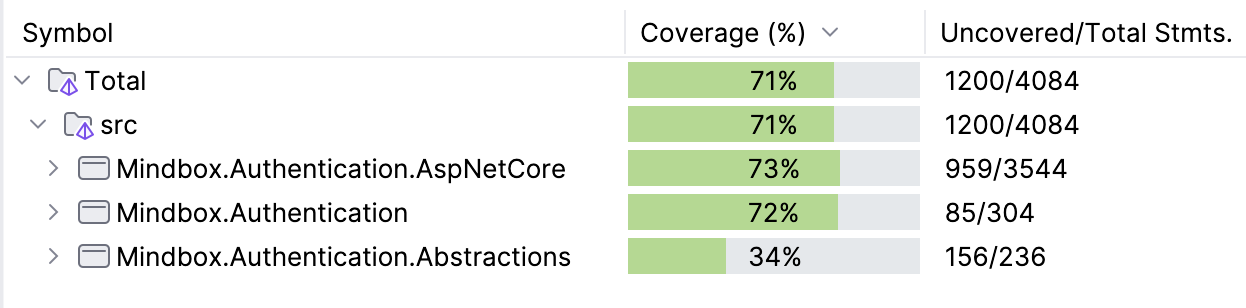
\includegraphics[width=\textwidth]{diagrams/img/lib-test-coverage.png}
  \caption{Покрытие кода тестами библиотеки Mindbox.Authentication}
  \label{fig:lib-test-coverage}
\end{figure}

\section{Выводы по главе}\label{sec:ch4-conclusion}

% TODO: апробация, нагрузочное тестирование, запуск ротации

\FloatBarrier
